\documentclass{article}
\usepackage{amsmath}
\usepackage{tikz}

\begin{document}

\[
\dot{H}^0(\mathbb{R}^n) = L^2(\mathbb{R}^n) \ (\gamma = 0)
\]

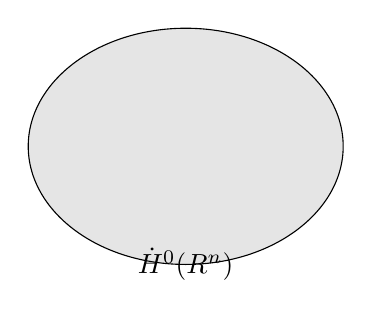
\begin{tikzpicture}[scale=1]
    % Define the ellipse parameters
    \def\rx{2} % x-radius
    \def\ry{1.5} % y-radius
    
    % Draw the ellipse
    \draw[fill=gray!20] (0,0) ellipse ({\rx} and {\ry});
    
    % Label the ellipse
    \node at (0,-1.5) {$\dot{H}^0(\mathbb{R}^n)$};
\end{tikzpicture}

\end{document}